%%%%%%%%%%%%%%%%%%%%%%%%%%%%%%%%%%%%%%%%%%%%%%%%%%%%%%%%%%%%%%%%%%%%
%%%%%%%%%%%%%%%%%%%%%%%%%%%%%%%%%%%%%%%%%%%%%%%%%%%%%%%%%%%%%%%%%%%%
%%                                                                %%
%% An example for writting your thesis using LaTeX                %%
%% Original version by Luis Costa,  changes by Perttu Puska       %%
%% Support for Swedish added 15092014                             %%
%%                                                                %%
%% This example consists of the files                             %%
%%         thesistemplate.tex (versio 2.01)                       %%
%%         opinnaytepohja.tex (versio 2.01) (for text in Finnish) %%
%%         aaltothesis.cls (versio 2.01)                          %%
%%         kuva1.eps                                              %%
%%         kuva2.eps                                              %%
%%         kuva1.pdf                                              %%
%%         kuva2.pdf                                              %%
%%                                                                %%
%%                                                                %%
%% Typeset either with                                            %%
%% latex:                                                         %%
%%             $ latex opinnaytepohja                             %%
%%             $ latex opinnaytepohja                             %%
%%                                                                %%
%%   Result is the file opinnayte.dvi, which                      %%
%%   is converted to ps format as follows:                        %%
%%                                                                %%
%%             $ dvips opinnaytepohja -o                          %%
%%                                                                %%
%%   and then to pdf as follows:                                  %%
%%                                                                %%
%%             $ ps2pdf opinnaytepohja.ps                         %%
%%                                                                %%
%% Or                                                             %%
%% pdflatex:                                                      %%
%%             $ pdflatex opinnaytepohja                          %%
%%             $ pdflatex opinnaytepohja                          %%
%%                                                                %%
%%   Result is the file opinnaytepohja.pdf                        %%
%%                                                                %%
%% Explanatory comments in this example begin with                %%
%% the characters %%, and changes that the user can make          %%
%% with the character %                                           %%
%%                                                                %%
%%%%%%%%%%%%%%%%%%%%%%%%%%%%%%%%%%%%%%%%%%%%%%%%%%%%%%%%%%%%%%%%%%%%
%%%%%%%%%%%%%%%%%%%%%%%%%%%%%%%%%%%%%%%%%%%%%%%%%%%%%%%%%%%%%%%%%%%%

%% Uncomment one of these:
%% the 1st when using pdflatex, which directly typesets your document in
%% pdf (use jpg or pdf figures), or
%% the 2nd when producing a ps file (use eps figures, don't use ps figures!).
\documentclass[english,12pt,a4paper,pdftex,sci,utf8]{aaltothesis}
%\documentclass[english,12pt,a4paper,dvips]{aaltothesis}

%% To the \documentclass above
%% specify your school: arts, biz, chem, elec, eng, sci
%% specify the character encoding scheme used by your editor: utf8, latin1

%% Use one of these if you write in Finnish (see the Finnish template):
%%
%\documentclass[finnish,12pt,a4paper,pdftex,elec,utf8]{aaltothesis}
%\documentclass[finnish,12pt,a4paper,dvips]{aaltothesis}

\usepackage{graphicx}
\usepackage[inkscapelatex=false]{svg}
\usepackage{tikz}


%% Use this if you write hard core mathematics, these are usually needed
\usepackage{amsfonts,amssymb,amsbsy, amsmath}


%% Use the macros in this package to change how the hyperref package below 
%% typesets its hypertext -- hyperlink colour, font, etc. See the package
%% documentation. It also defines the \url macro, so use the package when 
%% not using the hyperref package.
%%
%\usepackage{url}

%% Use this if you want to get links and nice output. Works well with pdflatex.
\usepackage[hidelinks]{hyperref}
\hypersetup{pdfpagemode=UseNone, pdfstartview=FitH,
  colorlinks=true,urlcolor=red,linkcolor=blue,citecolor=black,
  pdftitle={Default Title, Modify},pdfauthor={Your Name},
  pdfkeywords={Modify keywords}}

\usepackage{float}


%% All that is printed on paper starts here
\begin{document}

%% Change the school field to specify your school if the automatically 
%% set name is wrong
 \university{aalto University}
 \school{School of Science}

%% Only for B.Sc. thesis: Choose your degree programme. 
\degreeprogram{Computer Science}
%%


%% Valitse yksi näistä kolmesta
%%
%% Choose one of these:
\univdegree{BSc}
%\univdegree{MSc}
%\univdegree{Lic}

%% Your own name (should be self explanatory...)
\author{Daniel Michaeli}

%% Your thesis title comes here and again before a possible abstract in
%% Finnish or Swedish . If the title is very long and latex does an
%% unsatisfactory job of breaking the lines, you will have to force a
%% linebreak with the \\ control character. 
%% Do not hyphenate titles.
%% 

\thesistitle{A Review of GPU Acceleration Techniques in Option Pricing Models}
\place{Espoo}

%% For B.Sc. thesis use the date when you present your thesis. 
%% 
%% Kandidaatintyön päivämäärä on sen esityspäivämäärä! 
\date{16.2.2025}

%% B.Sc. or M.Sc. thesis supervisor 
%% Note the "\" after the comma. This forces the following space to be 
%% a normal interword space, not the space that starts a new sentence. 
%% This is done because the fullstop isn't the end of the sentence that
%% should be followed by a slightly longer space but is to be followed
%% by a regular space.
%%
\supervisor{M.Sc.\ Henrik Lievonen} %{Prof.\ Pirjo Professori}

%% B.Sc. or M.Sc. thesis advisors(s). You can give upto two advisors in
%% this template. Check with your supervisor how many official advisors
%% you can have.
%%
%\advisor{Prof.\ Pirjo Professori}
%\advisor{D.Sc.\ (Tech.) Olli Ohjaaja}
\advisor{M.Sc.\ Henrik Lievonen}

%% Aalto logo: syntax:
%% \uselogo{aaltoRed|aaltoBlue|aaltoYellow|aaltoGray|aaltoGrayScale}{?|!|''}
%%
%% Logo language is set to be the same as the document language.
%% Logon kieli on sama kuin dokumentin kieli
%%
\uselogo{aaltoBlack}{''}

%% Create the coverpage
%%
\makecoverpage


%% Note that when writting your master's thesis in English, place
%% the English abstract first followed by the possible Finnish abstract

%% English abstract.
%% All the information required in the abstract (your name, thesis title, etc.)
%% is used as specified above.
%% Specify keywords
%%
%% Kaikki tiivistelmässä tarvittava tieto (nimesi, työnnimi, jne.) käytetään
%% niin kuin se on yllä määritelty.
%% Avainsanat
%%
\keywords{moi, mojn, moin, morjens, moro}
%% Abstract text
\begin{abstractpage}[english]

English bla bla bla
\end{abstractpage}

%% Force a new page so that the possible English abstract starts on a new page
%%
%% Pakotetaan uusi sivu varmuuden vuoksi, jotta 
%% mahdollinen suomenkielinen ja englanninkielinen tiivistelmä
%% eivät tule vahingossakaan samalle sivulle
\newpage
%

%% Force new page so that the Swedish abstract starts from a new page
\newpage
%
%% Swedish abstract. Delete if you don't need it. 
%% 
\thesistitle{Genomströmning och latens i datorsystem: en anlays av avvägningseffekter och optimeringsstrategier}
\advisor{M.Sc.\ Henrik Lievonen} %
\degreeprogram{Datateknik}
\department{Högskolan för teknikvetenskaper}%
\professorship{?}  %
%% Abstract keywords
\keywords{Nyckelord p\aa{} svenska,\\ Moi, moin, moidå, mojjdå}
%% Abstract text
\begin{abstractpage}[swedish]
 svenska bla bla bla
\end{abstractpage}

\newpage


%% Table of contents. 

\thesistableofcontents




%% Tweaks the page numbering to meet the requirement of the thesis format:
%% Begin the pagenumbering in Arabian numerals (and leave the first page
%% of the text body empty, see \thispagestyle{empty} below).
%% Additionally, force the actual text to begin on a new page with the 
%% \clearpage command.
%% \clearpage is similar to \newpage, but it also flushes the floats (figures
%% and tables).
%% There is no need to change these
%%
\cleardoublepage
\storeinipagenumber
\pagenumbering{arabic}
\setcounter{page}{1}


%% Text body begins. Note that since the text body
%% is mostly in Finnish the majority of comments are
%% also in Finnish after this point. There is no point in explaining
%% Finnish-language specific thesis conventions in English. Someday 
%% this text will possibly be translated to English.
%%
\section{Introduction}

%% Ensimm\"ainen sivu tyhj\"aksi
%% 
%% Leave first page empty
\thispagestyle{empty}
Options are a type of financial contract between two parties that grants the right - but not the obligation - to buy or sell a specific amount of an asset at a predetermined price by a specific future date \cite[p. 6]{hull2016options}. Options are a type of financial derivative, meaning that their value depends on the value of an underlying asset. Advances in both financial mathematics \cite{merton1994influence} and affordable computational power \cite{nordhaus2007two} have driven rapid growth in the derivatives market by improving pricing models and risk management tools. The use of derivatives has increased significantly in the last 50 years, not only among investors but also among so-called nonfinancial corporations \cite{bartram2009international}. The use of options and other derivatives allows for both levered speculation and sophisticated investment and risk management strategies by providing finer exposure control.

There are many different option pricing models, each with their pros and cons, and based on different underlying assumptions. Regardless of the choice of model, the importance of speed remains critical. All else being equal, faster computation leads to improved decision-making in investing and risk management because of either executing faster, having more data available, or both. This has led to the interest in re-implementing common option pricing models to run, either in part or fully, on the graphics processing unit (GPU) due to its powerful parallel processing capabilities compared to the central processing unit (CPU).

This thesis forms a literature review of common option pricing models' GPU acceleration potential and limitations. The aim is to assess how dependency structures in different models affect their GPU parallelization potential, what models see the greatest performance improvements of a GPU implementation, analyze the scalability of these solutions in terms of both time and space complexity, and identify related challenges and bottlenecks. For simplicity, the following three models / methods have been chosen: the Cox-Ross-Rubinstein (CRR) binomial model, the Black-Scholes-Merton (BSM), and Monte Carlo (MC) simulation-based methods. Section~\ref{sec:optionfundamentals} introduces formal definitions and the fundamental mathematics of option pricing. Section~\ref{sec:gpu-computing} presents a high-level overview of the GPU, how it differs architecturally from the CPU, and how it can be used for general-purpose computing. Sections ~\ref{sec:gpu-crr}, ~\ref{sec:gpu-bsm} model, and ~\ref{sec:gpu-mc} review GPU implementation attempts of each respective model group, considering the aforementioned factors. The results are summarized in Section ~\ref{sec:summary} and conclusions are drawn in section ~\ref{sec:conclusions}.


For scope restriction purposes, the following choices have been made:
\begin{itemize}
    \item Only European and American style (vanilla) options are considered, with the exception of the Monte Carlo methods, which are particularly suitable for pricing exotic options with complex payoff structures. I will use the term "vanilla options" throughout the thesis to refer to both European and American style options (to be presented), whereas "exotic options" refer to more complex contracts. Unless explicitly stated otherwise, all discussions and conclusions apply to options in general. When specific terms are used, the statements pertain strictly to those contract styles.
    
    \item The purpose of this paper is to draw general conclusions about the GPU acceleration potential for different model groups. The referenced research uses varying microprocessor architectures and performance metrics. Other differences, like the number of active cores in the baseline CPU implementation, or the extent to which further optimization in e.g. memory access patterns have been implemented, also play a role. Thus, it must be acknowledged that direct quantitative comparisons are not always possible. Instead, I intend to incorporate the data into a more holistic, qualitative assessment that also considers the other factors of scalability and implementation difficulty.

    \item The models and implementations are studied purely from a computing performance perspective. That is, no interest is taken in the analysis of accuracy, conformity to assumptions, or any other unrelated aspect. The main comparisons of interest are the relative speedups of the GPU-accelerated implementations compared to a baseline solution, and to a smaller extent relative performance comparisons between different GPU-accelerated implementations.
\end{itemize}


%% Opinn\"aytteess\"a jokainen osa alkaa uudelta sivulta, joten \clearpage
%%
%% In a thesis, every section starts a new page, hence \clearpage
\clearpage

\section{Option Pricing Fundamentals} \label{sec:optionfundamentals}

The following section presents a sufficient theoretical introduction to options. Firstly, general definitions are established, after which 
vanilla option payoff functions are examined. Next, the risk-neutral valuation framework is presented, (non-rigorously) explaining the mathematical principles that underpin all major pricing models. This is followed by a subsection on the key determinants that influence option prices, and the sensitivity measures, known as "the Greeks", that quantify how prices change in response to these determinants. The section concludes with a discussion on the inherent computational challenges of option pricing, further motivating the exploration of GPU acceleration techniques.


\subsection{Definitions}
Chapter 1.5 in \cite{hull2016options} presents the following useful definitions and related terminology:

\paragraph{Call Option:}Grants the holder the right (but not the obligation) to buy the underlying asset by a certain date for a certain price.

\paragraph{Put Option:}Grants the holder the right (but not the obligation) to sell the underlying asset by a certain date for a certain price.

\paragraph{Strike Price:}The predetermined price at which the underlying asset can be bought (for a call option) or sold (for a put option) upon exercise.

\paragraph{Maturity (date):}The predetermined date on which the option expires, determining the latest point at which it can be exercised.
\bigskip

Note the ambiguous use of "by", as the specific rules for when an option can be exercised depends on the style of option. For our vanilla options, a European-style option must be exercised on the maturity date, whereas an American-style option can be exercised at any time up to the maturity.

There are always two parties to every option contract: the investor (buyer), who takes the \textbf{long} position, pays an up front premium to the underwriter (seller) for the right to engage in a future trade. Conversely, the underwriter, who takes the \textbf{short} position, now has an obligation to engage in this trade, and thus incurs a risk. A single option contract is considered a zero-sum game between the investor and the underwriter. Thus, we have a pair of mirrored positions for both a call option and a put option. These can be visualized by graphing the profit of each position at the time of exercising as a function of the underlying asset price. Alternatively, one can consider the slightly modified \textbf{payoff} of the position, which adds the premium back to the profit to focus only on the fundamental mechanics of the option itself:
\begin{equation}
    \text{profit}=\text{payoff}-\text{premium}
\end{equation}

\subsection{Vanilla Option Payoff Structures}\label{payoffs}


In a similar fashion to \cite[pp. 7-10]{hull2016options}, profit diagrams for each vanilla option position is presented below, along with practical examples for intuition. We consider European-style options for simplicity, but the profit diagrams for American-style options are identical as we only add the option of exercising earlier than at maturity. The options are based on one unit of the underlying asset. Transaction costs have been ignored. Let $p$ be the premium, or price paid for the option, $K$ the strike price, and $S_T$ the price of the underlying asset at maturity.



\subsubsection{Call Option Positions}
The investor is willing to pay a premium up front in order to fix a price for buying at a later time. In other words, they expect the price of the underlying asset to increase enough to offset this premium. Figure ~\ref{fig:long_call_payoff} depicts the profit diagram of a long position of a call option:

\begin{center}
\begin{figure}[H]
\centering
    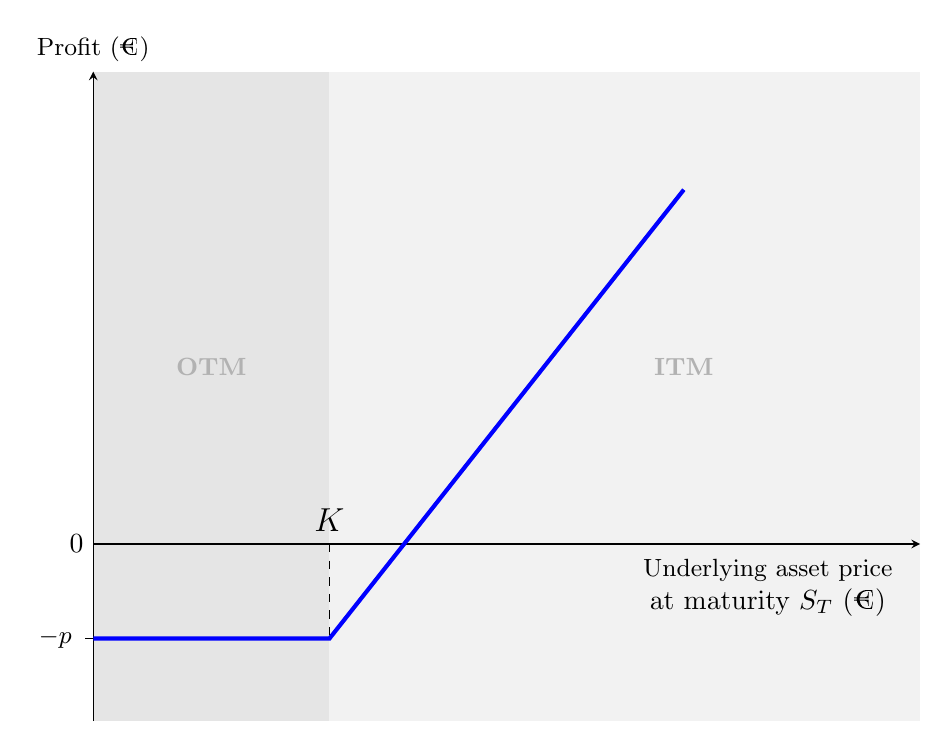
\begin{tikzpicture}[scale=1.5, >=stealth]

        % Shade area to the right of K (extending fully up to x-axis)
        \fill[gray!10] (2,-1.5) -- (7,-1.5) -- (7,4) -- (2,4) -- cycle;

         % Shade area to the left of K (extending fully up to x-axis)
        \fill[gray!20] (0,-1.5) -- (2,-1.5) -- (2,4) -- (0,4) -- cycle;


        % Define axes (extended x-axis)
        \draw[->] (0,0) -- (7,0) node[below,xshift=-55,yshift=-2pt, align=center] {\small Underlying asset price \\ at maturity $S_T$ (€)};
        \draw[->] (0,-1.5) -- (0,4) node[above] {\small Profit (€)};
        
        
        % Strike price line
        \draw[dashed] (2,0) -- (2,-0.8) node[above, yshift=35] {\large$K$};
        
        % Payoff function (thicker blue line)
        \draw[line width=1.5pt, blue] (0,-0.8) -- (2,-0.8) -- (5,3);
        
        % Marking zero level
        \node[left] at (0,0) {0};
        
        % Adding the premium annotation
        \draw (-0.07,-0.8) -- (0,-0.8); % Short tick line
        \node[left] at (-0.1,-0.8) {\small $-p$};

        % Add "ITM" label inside the fully shaded area
        \node[gray!60] at (5,1.5) {\small \textbf{ITM}};

        % Add "OTM" label inside the fully shaded area
        \node[gray!60] at (1,1.5) {\small \textbf{OTM}};

    \end{tikzpicture}
    \caption{Profit diagram for a long call option. $K$ = strike price, $p$ = premium}
    \label{fig:long_call_payoff}
\end{figure}
\end{center}

As long as $S_T$ < $K$ we are at a net loss equal to the paid premium $p$. The option is said to be \textbf{out of the money (OTM)}, and has no intrinsic value. When $S_T = K$ the option is considered to be \textbf{at the money (ATM)}, after which, when $S_T > K$ it is \textbf{in the money (ITM)} and has some intrinsic value, or a positive payoff \cite[p. 209]{hull2013fundamentals}. Still, the profit remains negative as long as payoff < $p$. Only  after offsetting the premium does the option truly become profitable for the investor. Note that the "moneyness" terminology is defined from the perspective of the long (investor's) position. Assuming liquid markets, they could then exercise the option to buy the underlying asset for the strike price, only to immediately sell for the current market price to profit off the difference. In general, ITM options are exercised, as the intrinsic value helps to offset at least some of the loss incurred from paying the premium.  

To demonstrate options' role in risk management as opposed to pure speculation, consider a company that relies heavily on crude oil for their manufacturing. If they expect a sharp increase in oil prices in a year from now they might choose to enter a long position in a call option with the oil distributor. The manufacturer knows it cannot afford the projected oil prices, and is willing to pay a premium in order to hedge against that risk.

At the other side of the contract the underwriter takes the short position, initially receiving the premium. They expect the price of the underlying asset not to rise too high above market value, as they are then obligated to sell the underlying asset at a price lower than market value, potentially offsetting the premium. Figure ~\ref{fig:short_call_payoff} depicts the corresponding profit diagram:

\begin{center}
\begin{figure}[H]
\centering
    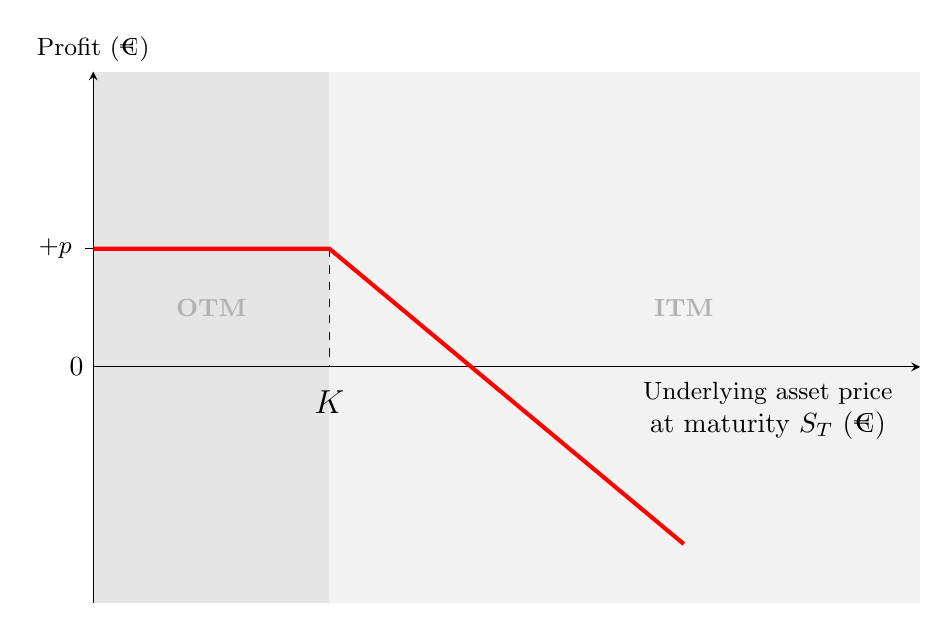
\begin{tikzpicture}[scale=1.5, >=stealth]

        % Shifted coordinate system for better x-axis positioning
        \begin{scope}[shift={(0,2)}]  

            % Shade area to the right of K (ITM for short call)
            \fill[gray!10] (2,2.5) -- (7,2.5) -- (7,-2) -- (2,-2) -- cycle;

            % Shade area to the left of K (OTM for short call)
            \fill[gray!20] (0,2.5) -- (2,2.5) -- (2,-2) -- (0,-2) -- cycle;

            % Define axes (extended x-axis, now moved up)
            \draw[->] (0,0) -- (7,0) node[below,xshift=-55,yshift=-2pt, align=center] {\small Underlying asset price \\ at maturity $S_T$ (€)};
            \draw[->] (0,-2) -- (0,2.5) node[above] {\small Profit (€)};
        
            % Strike price line
            \draw[dashed] (2,1) -- (2,0) node[below, yshift=-5] {\large$K$};
        
            % Payoff function (thicker red line for short call)
            \draw[line width=1.5pt, red] (0,1) -- (2,1) -- (5,-1.5);

            % Marking zero level
            \node[left] at (0,0) {0};
        
            % Adding the premium annotation (shifted higher)
            \draw (-0.07,1) -- (0,1); % Short tick line
            \node[left] at (-0.1,1) {\small $+p$};

            % Add "ITM" label inside the shaded area (short call ITM is left of K)
            \node[gray!60] at (1,0.5) {\small \textbf{OTM}};

            % Add "OTM" label inside the shaded area (short call OTM is right of K)
            \node[gray!60] at (5,0.5) {\small \textbf{ITM}};

        \end{scope}
    \end{tikzpicture}
    \caption{Profit diagram for a short call option. $K$ = strike price, $p$ = premium}
    \label{fig:short_call_payoff}
\end{figure}
\end{center}

An inverse behavior is observed: as long as the option remains OTM (or at most ATM) the underwriter is guaranteed a profit equal to the premium, as the investor will not exercise the option. Once the option becomes ITM the investor will exercise it, and the underwriter will be forced to sell the underlying asset at a lower price than market value. As long as the loss of this trade is small enough, the premium will offset it, yielding a positive profit. The option truly becomes a loss when the breakeven point is reached. Continuing with the previous example, this could be the position taken by a crude oil producer with confidence that the prices will not greatly exceed the strike price in a year's time.

Ignoring the premium, the payoff from the long position in a call option is defined as

\begin{equation}
    \max(S_T-K,0)
\end{equation}

as the investor will only exercise when ITM to either profit or offset losses. The payoff from the short position is defined as


\begin{equation}
    -\max(S_T-K,0) = \min(K-S_T,0)
\end{equation}

due to the zero-sum nature of the contract \cite[p. 9]{hull2016options}. \textbf{DO I NEED PAYOFF GRAPHS?? THEY'RE VERY SIMILAR}

\subsubsection{Put Option Positions}
The investor is willing to pay a premium up front in order to fix a price for selling a later time. In other words, they expect the price of the underlying asset to decrease enough to offset this premium. Meanwhile, the underwriter receives a premium but is obligated to engage in this potential future trade, and thus expects the price not to decrease too much from the market price. Figure ~\ref{fig:put_payoff} depicts the profit diagrams of the long and short positions of a put option:


\begin{figure}[H]
    \makebox[\textwidth][c]{
    \hspace{-1cm} % Fine-tune centering
    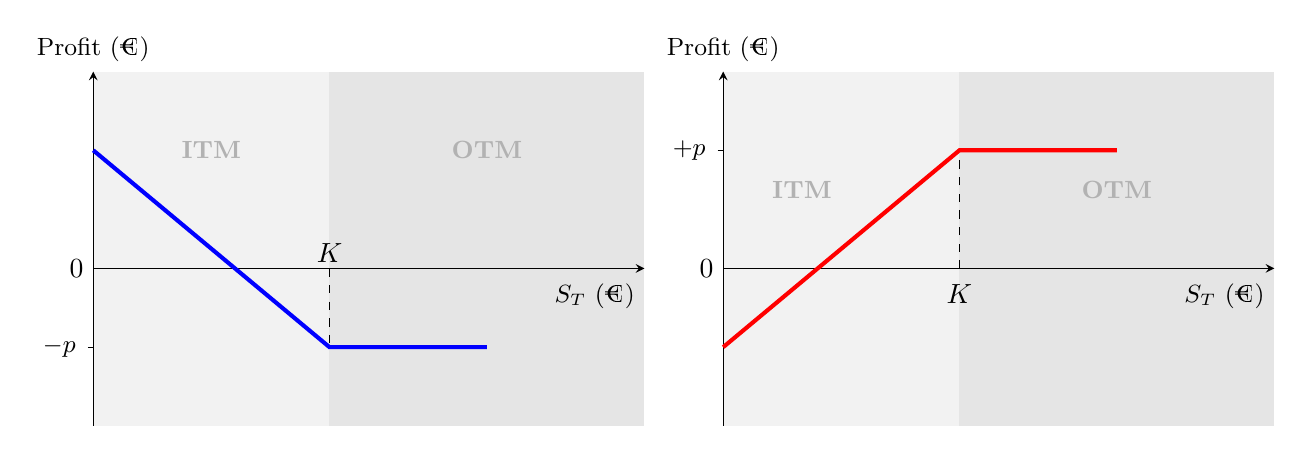
\begin{tikzpicture}[scale=1, >=stealth]

     % Left Diagram: Long Put
    \begin{scope}[shift={(-0.5,2)}]  % Shifted slightly left

        % Shade area to the right of K (OTM for long put)
        \fill[gray!20] (3,2.5) -- (7,2.5) -- (7,-2) -- (3,-2) -- cycle;

        % Shade area to the left of K (ITM for long put)
        \fill[gray!10] (0,2.5) -- (3,2.5) -- (3,-2) -- (0,-2) -- cycle;

        % Define axes
        \draw[->] (0,0) -- (7,0) node[below,xshift=-18,yshift=-2pt, align=center] {\small$S_T$ (€)};
        \draw[->] (0,-2) -- (0,2.5) node[above] {\small Profit (€)};
    
        % Strike price line
        \draw[dashed] (3,0) -- (3,-1) node[above, yshift=27] {$K$};
    
        % Payoff function (thicker blue line for long put)
        \draw[line width=1.5pt, blue] (0,1.5) -- (3,-1) -- (5,-1);%(0,1.5) -- (2,1.5) -- (5,-1);

        % Marking zero level
        \node[left] at (0,0) {0};
    
        % Adding the premium annotation
        \draw (-0.07,-1) -- (0,-1); % Short tick line
        \node[left] at (-0.1,-1) {\small $-p$};

        % Add "ITM" label inside the shaded area (long put ITM is left of K)
        \node[gray!60] at (1.5,1.5) {\small \textbf{ITM}};

        % Add "OTM" label inside the shaded area (long put OTM is right of K)
        \node[gray!60] at (5,1.5) {\small \textbf{OTM}};

    \end{scope}

    % Right Diagram: Short Put (Shifted slightly left from 9 to 8)
    \begin{scope}[shift={(7.5,2)}]  

        % Shade area to the right of K (ITM for short put)
        \fill[gray!20] (2,2.5) -- (7,2.5) -- (7,-2) -- (2,-2) -- cycle;

        % Shade area to the left of K (OTM for short put)
        \fill[gray!10] (0,2.5) -- (3,2.5) -- (3,-2) -- (0,-2) -- cycle;

        % Define axes
        \draw[->] (0,0) -- (7,0) node[below,xshift=-18,yshift=-2pt, align=center] {\small$S_T$ (€)};
        \draw[->] (0,-2) -- (0,2.5) node[above] {\small Profit (€)};
    
        % Strike price line
        \draw[dashed] (3,0) -- (3,1.5) node[below,yshift=-45] {$K$};
    
        % Payoff function (thicker red line for short put)
        \draw[line width=1.5pt, red] (0,-1) -- (3,1.5) -- (5,1.5);

        % Marking zero level
        \node[left] at (0,0) {0};
    
        % Adding the premium annotation
        \draw (-0.07,1.5) -- (0,1.5); % Short tick line
        \node[left] at (-0.1,1.5) {\small $+p$};

        % Add "OTM" label inside the shaded area (short put OTM is right of K)
        \node[gray!60] at (5,1) {\small \textbf{OTM}};

        % Add "ITM" label inside the shaded area (short put ITM is left of K)
        \node[gray!60] at (1,1) {\small \textbf{ITM}};

    \end{scope}

    \end{tikzpicture}

    
}
\caption{Profit diagrams: (Left) Long put option, (Right) Short put option.}
\label{fig:put_payoff}
\end{figure}

A put option is worthless (OTM) when $S_T > K$ as the investor will not exercise it to sell for a lower price than market value. By the same token, the option is ITM when  $S_T < K$, as the investor can then buy the underlying asset at market value and sell it for the strike price \cite[p. 209]{hull2013fundamentals}. Again, being ITM is not sufficient to be profitable - the price difference must be large enough to offset the paid premium.

An example use case would be a crude oil supplier forecasting low prices in a year's time and entering the long position to secure a minimum revenue. Again, a premium is paid to hedge against a risk of price swings. The short side would be taken by a market participant who expects crude oil prices not to fall enough to offset the received premium.
\bigskip

The payoff from the long position in a put option is defined as

\begin{equation}
    \max(K-S_T,0)
\end{equation}

as being ITM now means $K > S_T$. The payoff in the corresponding short position is

\begin{equation}
    -\max(K-S_T,0) = \min(S_T-K,0)
\end{equation}

due to the zero-sum nature of the contract \cite[p. 10]{hull2016options}.


Underlying asset prices are often theoretically unbounded, whereas the potential losses are limited (no negative prices). For this reason, taking the short position is inherently more risky as the potential losses are limitless. Table\ref{???} aggregates the information about the risk of taking different option positions.

INSERT TABLE HERE




\subsection{Price Determinants and Sensitivity}

Hull et. al. \cite{hull2013fundamentals} define six factors influencing the price of the option. While these often make up the variables in our pricing models, one can intuitively reason about their effect in a model-free context. This also, however, provides some explanation on why they appear in the models in the first place. They are presented in a "ceteris paribus" context (all else being equal). This is rarely the case in practice, however, as markets quickly incorporate available information into prices \cite{fama1970efficient}. The underlying asset price is consequently affected by changes in some of the factors. For clarity, we are considering the long position, i.e. the perspective of the buyer.

The stock price relative to the strike price is perhaps the most obvious factor. The effect on the payoff is thoroughly explained in subsection ~\ref{payoffs}, and the price naturally increases with the payoff. Thus, the price of a call option increases with the underlying asset, while the inverse relationship is observed for a put option.

Volatility, a statistical measure of the variation in asset prices over a specific time period, has a positive effect on both call and put options. This can be motivated by the limited downside - unlimited upside nature of options (SEE TABLE XXX), which makes larger price movements more advantageous as it increases the probability of moving ITM. This is especially obvious for OTM positions, where a price movement is still needed in order not to expire worthless, but holds for ITM positions as well, as the unlimited potential for becoming even deeper ITM outweighs the limited downside of going OTM.

Time to maturity has a more complex relationship with the price, and depends on both the option style and the context. For American-style options where early exercise is allowed, it makes sense that an expiration date further in the future leads to more opportunity for favorable movements in the underlying, thereby commanding a higher price. This is effectively the same argument as was made for  volatility. While this so called "time-decay" argument also holds for European-style options, the lack of early-exercise complicates the matter. There exist specific scenarios where one would benefit from exercising the option earlier. The authors propose the example of a future dividend payment to the shareholders of the underlying company, which theoretically decreases the share price and thereby the value of the corresponding call option. An example of a put option being of higher value with a shorter timer to maturity would be the case of a very deep ITM position, e.g. if the company of the underlying asset has filed for bankruptcy. The option will almost certainly expire ITM, and thus by the \textbf{time value of money} principle this cash flow is worth more the earlier it is received \cite[pp. 97-101]{berk2007corporate}.


The risk-free rate represents the return on investment one can expect from a so called risk-free investment. In practice, this means some form of government-backed treasury bill (as the government is "too big to fail"). It often serves as a sort of benchmark measurement to which investors compare the expected rates of return of other, riskier investments. Given a risk level for an investment, an increase in the risk-free rate leads to investors expecting a higher return on said investment. Consequently, since the expected rate of return is often used as the discount rate for obtaining the present value of future cash flows, it decreases the present value of the strike price, which, all else being equal, is a better deal for the buyer and increases the value of the call option. By the same token, the value of a put option decreases, as the strike price is "worth more" by maturity than what it is in today's money. In practice, however, interest rates tend to have a notable and varying impact on different underlying asset prices as well, so this is more of a theoretical relationship assuming a standard share as the underlying.

The final determinant considers the dividend policy of the underlying asset (stock). Theoretically, a company's share price is reduced by the dividend, as this money is directly deducted from the cash flows that make up the value of the equity in the first place \cite{modigliani1958cost}. Thus, a dividend payment policy decreases the value of a call option, and increases the value of a put option.

In addition to pricing the option, traders and risk managers alike are often interested in measuring how sensitive this price is to changes in these determinants. Model imperfections make it desirable to understand the effect of small perturbation in the variables, hence these often play a significant role in different hedging and trading strategies \cite{hull2016options}. Wilmott \cite{wilmott2013paul} defines the following five main sensitivity measures, also known as \emph{the Greeks}, with respect to the aforementioned determinants. \bigskip \\Let $V$ be the price (value) of the option, $S$ the underlying asset price, $t$ the time to maturity, $r$ the risk-free rate, and $\sigma$ the volatility of the underlying asset. A high-level definition of the Greeks is:
\begin{align*}
    \Delta &= \frac{\partial V}{\partial S} & \text{(Delta: sensitivity to changes in the underlying price)} \\[0.5em]
    \Gamma &= \frac{\partial^2 V}{\partial S^2} & \text{(Gamma: rate of change of Delta, or convexity)} \\[0.5em]
    \Theta &= \frac{\partial V}{\partial t} & \text{(Theta: sensitivity to the passage of time)} \\[0.5em]
    \nu &= \frac{\partial V}{\partial \sigma} & \text{(Vega: sensitivity to volatility changes)} \\[0.5em]
    \rho &= \frac{\partial V}{\partial r} & \text{(Rho: sensitivity to changes in the risk-free rate)}
\end{align*}

Note that the formal definitions of the Greeks are model-specific. The choice to represent them using partial derivatives suggests the context of a continuous-time model, and are indeed defined in relation to the BSM model. Nevertheless, this formulation provides an intuitive understanding of the measurements. In discrete-time models (like CRR) or discretized approximations of BSM, the Greeks are redefined or estimated using different techniques (do I need sources???).


\subsection{Risk-Neutral Valuation Framework}
- the choice of option pricing model really is the choice of how to model the underlying asset's price behavior
\subsubsection{Replicating portfolio and no-arbitrage principle}
\subsection{risk-neutral derivation, and how it manifests in our three model groups}

\subsection{The Greeks}

\subsection{Computational Challenges in Option Pricing}


\section{The GPU and Parallel Computing} \label{sec:gpu-computing}
\subsection{CPU vs. GPU Architecture}

Traditional CPU design philosophy
GPU architectural principles
SIMD vs. SIMT execution models
Memory hierarchy differences

\subsection{GPU Programming Model}

Thread hierarchy (threads, blocks, grids)
Memory spaces (global, shared, constant, texture)
Execution model and scheduling
CUDA/OpenCL programming paradigms

\subsection{Parallel Computing Fundamentals and GPU suitability}

Types of parallelism (data, task, instruction)
Amdahl's Law and theoretical speedup limits
Dependency chains and their impact
Synchronization requirements
Characteristics of "GPU-friendly" algorithms
Identifying parallelizable components
Common computation patterns in finance
Performance metrics and evaluation

\subsection{Performance Considerations} ???

Memory transfer bottlenecks
Thread divergence
Coalesced memory access
Occupancy optimization
Warp efficiency

\clearpage

\section{GPU Acceleration of the Cox-Ross-Rubinstein Binomial Model} \label{sec:gpu-crr}
\subsection{Binomial}
\subsection{Trinomial}
\subsection{???}

\section{GPU Acceleration of the Black-Scholes-Merton Model} \label{sec:gpu-bsm}
\subsection{Black-Scholes-Merton Model Framework}
\subsection{European option analytical solution GPU vs CPU}
\subsection{Finite Differences numerical method for??}
\subsection{???}

\section{GPU Acceleration of Monte Carlo Methods} \label{sec:gpu-mc}
\subsection{MC in general}
\subsection{MC in options' theory}
\subsection{??????}

T\"ass\"a osassa kuvataan k\"aytetty tutkimusaineisto ja
tutkimuksen metodologiset valinnat, sek\"a
kerrotaan tutkimuksen toteutustapa ja k\"aytetyt menetelm\"at. 

\clearpage


%% Huomaa seuraavassa kappaleessa lainausmerkkien ulkopuolella piste, 
%% koska piste ei lopeta lainattua tekstinp\"atk\"a\"a.
%% Jos lainattu tekstinp\"atk\"a loppuu v\"alimerkkiin, tulee v\"alimerkki
%% lainausmerkkien sis\"alle: 
%% "Et tu, Brute?" sanoi Caesar kuollessaan.
Tutkimustuloksien merkityst\"a on aina syyt\"a arvioida ja tarkastella
kriittisesti.  Joskus tarkastelu voi olla t\"ass\"a osassa, mutta se
voidaan my\"os j\"att\"a\"a viimeiseen osaan, jolloin viimeisen osan nimeksi
tulee >>Tarkastelu>>. Tutkimustulosten merkityst\"a voi arvioida my\"os
>>Johtop\"a\"at\"okset>>-otsikon alla viimeisess\"a osassa. 

T\"ass\"a osassa on syyt\"a my\"os arvioida tutkimustulosten luotettavuutta.
Jos tutkimustulosten merkityst\"a arvioidaan >>Tarkastelu>>-osassa,
voi luotettavuuden arviointi olla my\"os siell\"a. 

\clearpage

\section{Summary}  \label{sec:summary}

\section{Conclusions}  \label{sec:conclusions}


Opinn\"aytteen tekij\"a vastaa siit\"a, ett\"a opinn\"ayte on t\"ass\"a dokumentissa
ja opinn\"aytteen tekemist\"a k\"asittelevill\"a luennoilla sek\"a
harjoituksissa annettujen ohjeiden mukainen muotoseikoiltaan,
rakenteeltaan ja ulkoasultaan.\cite{grochowski2004best}


\cleardoublepage
\phantomsection

\addcontentsline{toc}{chapter}{\bibname}
\bibliographystyle{IEEEtran}
\bibliography{bibliography.bib}


\end{document}